\documentclass{jsarticle}
\usepackage[dvipdfmx]{graphicx}
\usepackage{bm}
\usepackage{amsmath}
\usepackage{amssymb}
\usepackage{amsfonts}
\usepackage{comment}
\usepackage{listings}
\usepackage{cases}
\lstset{
    basicstyle={\ttfamily},
    identifierstyle={\small},
    commentstyle={\smallitshape},
    keywordstyle={\small\bfseries},
    ndkeywordstyle={\small},
    stringstyle={\small\ttfamily},
    frame={tb},
    breaklines=true,
    columns=[l]{fullflexible},
    numbers=left,
    xrightmargin=0zw,
    xleftmargin=3zw,
    numberstyle={\scriptsize},
    stepnumber=1,
    numbersep=1zw,
    lineskip=-0.5ex,
    keepspaces=true,
    language=c
}
\renewcommand{\lstlistingname}{リスト}
\makeatletter
\newcommand{\figcaption}[1]{\def\@captype{figure}\caption{#1}}
\newcommand{\tblcaption}[1]{\def\@captype{table}\caption{#1}}
\makeatother

\title{数値解析レポートNo.4}
\author{32番 平田 蓮}
\date{}

\begin{document}
\maketitle
    \section{連立微分方程式}
        \begin{eqnarray}
            f(x, y; t) &=& \frac{dx}{dt} = x + 6y + t - 10 \nonumber \\
            g(x, y; t) &=& \frac{dy}{dt} = x + t - 3 \nonumber
        \end{eqnarray}

        とすると、$x, y$の値をオイラー法のように解くことができる。
        具体的には以下の式を実装すれば良い。

        \begin{eqnarray}
            x_{i + 1} &=& x_i + f(x_i, y_i; t)dt \nonumber \\
            y_{i + 1} &=& y_i + g(x_i, y_i; t)dt \nonumber
        \end{eqnarray}

        リスト\ref{src:sim}に二連立微分方程式を解く関数\verb|sim_euler()|を示す。

        \begin{lstlisting}[caption=sim\_euler.c, label=src:sim]
#define N 10000

void sim_euler(
    double (*f)(
        double x, double y, double t
    ),
    double (*g)(
        double x, double y, double t
    ),
    double x[N],
    double y[N],
    double l,
    double r,
    int n,
    int debug
) {
    double t = 0, dt = (l + r) / (double)n;
    int i;

    for (i = 1; i <= n; i++, t += dt) {
        if (debug) {
            printf("t: %4.4f, x: %4.4f, y: %4.4f\n", t, x[i - 1], y[i - 1]);
        }

        x[i] = x[i - 1] + f(x[i - 1], y[i - 1], t) * dt;
        y[i] = y[i - 1] + g(x[i - 1], y[i - 1], t) * dt;
    }

    if (debug) {
        printf("t: %4.4f, x: %4.4f, y: %4.4f\n", t, x[n], y[n]);
    }
}\end{lstlisting}

        この関数を用いて$x, y$の解を求めたものを図\ref{fig:simx}, \ref{fig:simy}に示す。

        \begin{figure}[h]
            \begin{minipage}{0.5\hsize}
                \centering
                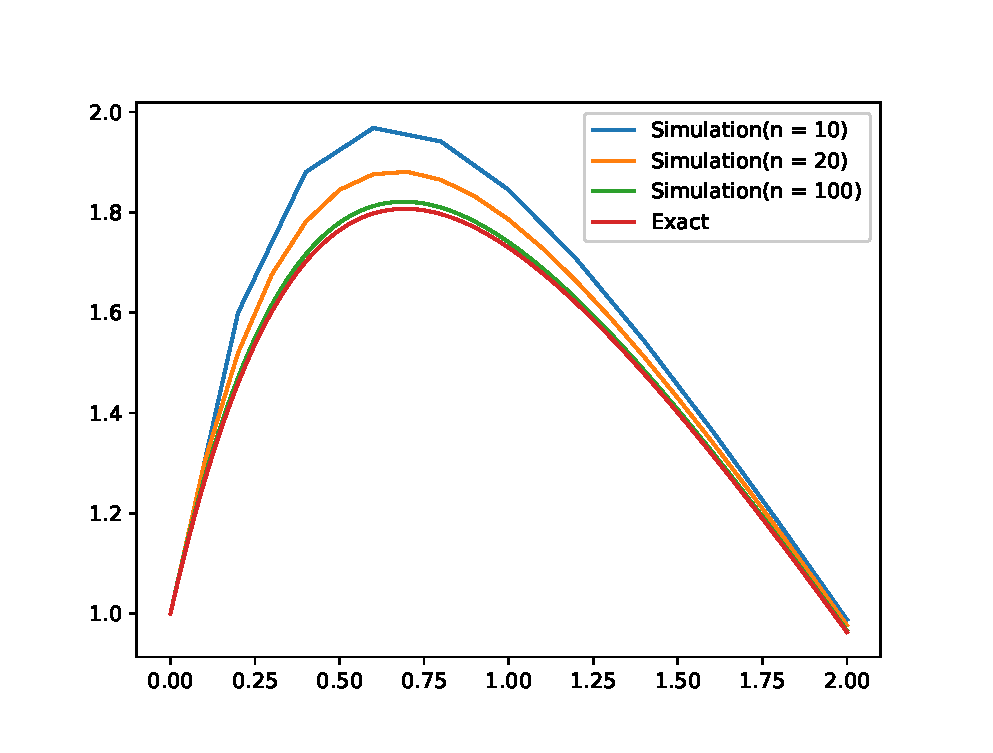
\includegraphics[width=1\hsize]{img/x.eps}
                \caption{$x$の解}
                \label{fig:simx}
            \end{minipage}
            \begin{minipage}{0.5\hsize}
                \centering
                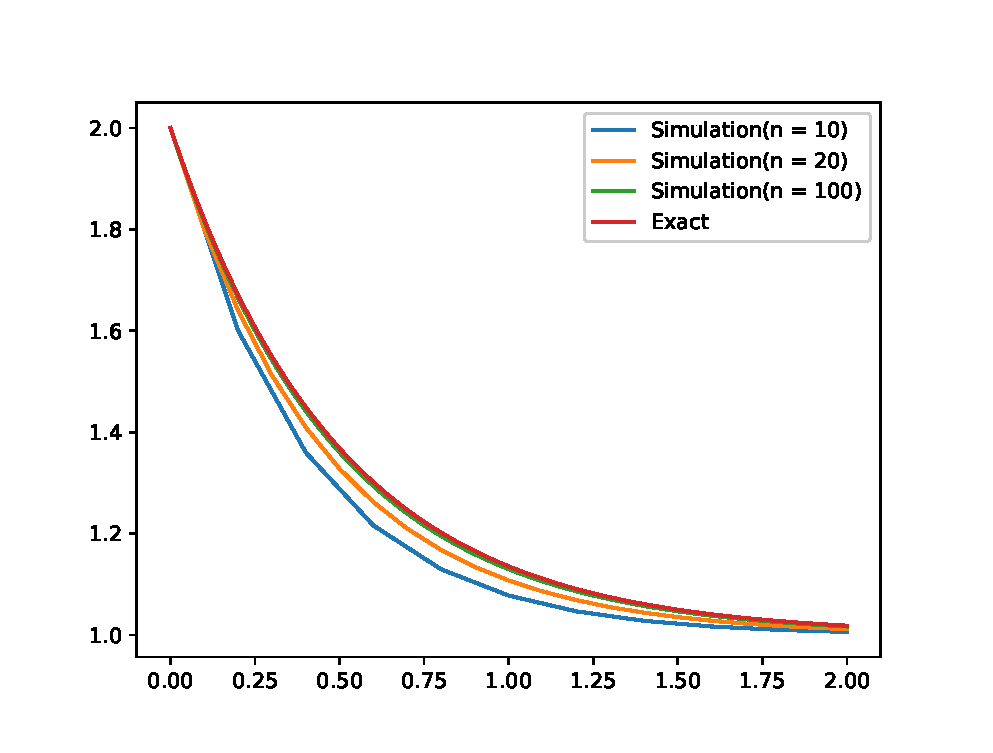
\includegraphics[width=1\hsize]{img/y.eps}
                \caption{$y$の解}
                \label{fig:simy}
            \end{minipage}
        \end{figure}

        ステップ幅を狭めるほど正確な近似ができていることがわかる。

    \section{高次微分方程式}
        $\displaystyle\frac{d^2y}{dx^2}+5\frac{dy}{dx}-6y=0$について、
        $\displaystyle\frac{dy}{dx}=z$とすることで,
        以下のように二次連立微分方程式とできる。

        \begin{eqnarray}
            \frac{dz}{dx} &=& 6y-5z \nonumber \\
            \frac{dy}{dx} &=& z \nonumber
        \end{eqnarray}

        これは前節と同じように解くことができる。
        $y$の解を図\ref{fig:high}に示す。

        \begin{figure}[h]
            \centering
            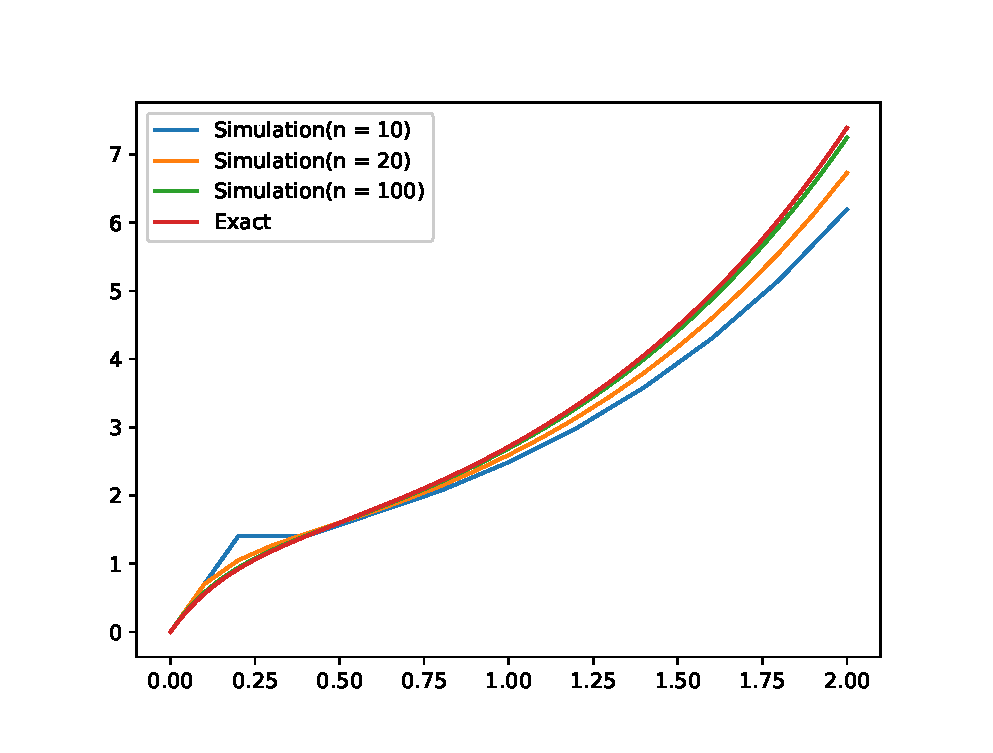
\includegraphics[width=0.8\hsize]{img/y2.eps}
            \caption{$y$の解}
            \label{fig:high}
        \end{figure}

        分割数$n=100$のとき、$x=1$に対して$y\approx 2.72$である。

    \section{考察}
        どちらの微分方程式も、オイラー法の式を使い同様に解いたが、
        ホイン法の漸化式を使うと精度が高まることが考えられる。

        また、今回作成したプログラムは二連立にしか対応していないが、
        任意個数の引数を受け取る関数を作ることで$n$連立に対応させられると考えられる。
\end{document}